\chapter{O desenho da intervenção}\label{cap:desenho}

O capítulo anterior deixou duas explicações de pé para a mesma série. Numa, a oscilação de amanhã
depende do que a série fez hoje; na outra, existe um estado escondido trocando de lei sem aparecer
no que se vê. Nenhuma das quatro leituras do dado escolheu entre as duas, e a saída que sobra é
mexer no mundo de propósito.

\section{O experimento que não separa}

Mexer no mundo, aqui, tem uma forma só. A série vai a zero por decreto durante alguns dias --- o
mundo é segurado parado ---, e depois é solta. Nada mais muda: a mesma lei, o mesmo relógio, a
mesma escala.

O experimento que vem à cabeça é segurar por muito tempo, uma vez. Entre segurar e observar, cada
tentativa dessas custa \numDesenhoDiasPorReplicataMaior{} dias, e devolve um número sozinho, sem
com o que comparar. Feito duas vezes nos dois mundos empatados, esse experimento separa as
explicações em \numDesenhoSeparaPoucasPct\% das repetições: quem decide assim está decidindo no
sorteio, e vai decidir com ele.

Vale dizer onde o empate é apertado, porque é ali que a observação gastou tudo o que tinha. Contra
as quatro leituras do capítulo anterior, os dois mundos concordam dentro da tolerância declarada, e
a leitura que chega mais perto da borda é o pior bloco de sessenta dias:
\numDesenhoEmpatePiorDiferenca{} contra uma tolerância de \numDesenhoEmpateToleranciaPior{}. É a
mesma estatística que já era gargalo quando se procurou uma lei compartilhada entre mercados, e ela
reaparece aqui como a fronteira do que se consegue distinguir olhando.

Os dois mundos foram calibrados numa série de \numDesenhoDiasSerie{} dias, e as quatro leituras que
empatam são medianas sobre \numDesenhoSementesEmpate{} sementes cada. Os parâmetros dos dois mundos
são fixos no caderno, de modo que quem quiser repetir a medição repete também o empate.

\section{O ato e a resposta}

O mesmo ato significa coisas diferentes conforme o lugar onde a memória mora, e por isso a medida
precisa ser declarada antes de ser usada.

\begin{definicao}[contenção e resposta]\label{def:resposta}
Uma \emph{contenção} de $k$ dias fixa a série em zero durante $k$ dias consecutivos. A
\emph{resposta} do mundo a essa contenção é a média de $|x|$ nos $m$ dias seguintes à soltura,
dividida pela média de $|x|$ nos $m$ dias anteriores à contenção. Uma \emph{replicata} é um mundo
sorteado inteiro, segurado e observado uma vez.
\end{definicao}

A referência é o próprio mundo. Um mundo que volta ao que era responde $1$; um mundo que volta
ferido responde menos que $1$. Medir contra a escala de fora misturaria a ferida com o tamanho do
mundo, e os dois mundos têm o mesmo tamanho por construção.

O que separa as duas explicações é a forma da resposta. Onde a memória mora na série, segurar apaga
a memória: a oscilação cai enquanto o mundo está parado e precisa ser reconstruída depois, tanto
mais devagar quanto mais fundo o buraco. Onde o estado é escondido, o estado corre durante a
contenção: a série fica parada e a lei continua trocando, de modo que a soltura devolve o mundo no
ponto em que a lei estiver.

\begin{proposicao}[o piso da contenção]\label{prop:piso-contencao}
Num mundo cuja oscilação obedece $v(t) = \omega + \alpha\, x(t-1)^2 + \beta\, v(t-1)$, com
$\alpha > 0$ e $0 < \beta < 1$, a variância no $k$-ésimo dia de uma contenção é
\[
v(k) \;=\; \frac{\omega}{1-\beta} \;+\; \beta^{k}\Big( v(0) - \frac{\omega}{1-\beta} \Big),
\]
que decresce para o piso $\omega/(1-\beta)$. Esse piso é $\sigma^{2}\,(1-\alpha-\beta)/(1-\beta)$,
menor que a variância de repouso $\sigma^{2}$ sempre que $\alpha > 0$.
\end{proposicao}

\begin{proof}
Durante a contenção a série é zero, de modo que $x(t-1)^2 = 0$ e a recursão perde o termo da
observação: $v(t) = \omega + \beta\, v(t-1)$. Iterando $k$ vezes a partir de $v(0)$ chega-se à
forma fechada, e o limite quando $k$ cresce é o ponto fixo da recursão, $\omega/(1-\beta)$. A
variância de repouso é $\sigma^{2} = \omega/(1-\alpha-\beta)$, de modo que o piso dividido por
$\sigma^{2}$ é $(1-\alpha-\beta)/(1-\beta)$, que fica abaixo de um assim que $\alpha$ é positivo.
\end{proof}

A proposição entrega as duas peças que o desenho usa. A primeira: segurar mais fundo tem limite. A
oscilação não vai a zero, ela vai ao chão que o próprio mecanismo declara, e a partir dali a
resposta para de descer. A segunda: a profundidade se compra em $\beta^{k}$, de modo que cada dia a
mais de contenção compra menos ferida do que o anterior. Uma curva que satura não é um acidente da
medição; é a forma que a lei obriga.

\section{A medição}

\begin{table}[htbp]
  \centering
  \small
  \begin{tabular}{rrrrr}
    \hline
    contenção & resposta da & resposta do estado & diferença & dias de \\
    (dias) & memória na série & escondido & medida & experimento \\
    \hline
    um & \numDesenhoRespostaMemoriaUm & \numDesenhoRespostaEscondidoUm & \numDesenhoDiferencaUm & \numDesenhoCustoUm \\
    dois & \numDesenhoRespostaMemoriaDois & \numDesenhoRespostaEscondidoDois & \numDesenhoDiferencaDois & \numDesenhoCustoDois \\
    cinco & \numDesenhoRespostaMemoriaCinco & \numDesenhoRespostaEscondidoCinco & \numDesenhoDiferencaCinco & \numDesenhoCustoCinco \\
    dez & \numDesenhoRespostaMemoriaDez & \numDesenhoRespostaEscondidoDez & \numDesenhoDiferencaDez & \numDesenhoCustoDez \\
    vinte & \numDesenhoRespostaMemoriaVinte & \numDesenhoRespostaEscondidoVinte & \numDesenhoDiferencaVinte & \numDesenhoCustoVinte \\
    quarenta & \numDesenhoRespostaMemoriaQuarenta & \numDesenhoRespostaEscondidoQuarenta & \numDesenhoDiferencaQuarenta & \numDesenhoCustoQuarenta \\
    oitenta & \numDesenhoRespostaMemoriaOitenta & \numDesenhoRespostaEscondidoOitenta & \numDesenhoDiferencaOitenta & \numDesenhoCustoOitenta \\
    cento e sessenta & \numDesenhoRespostaMemoriaCentoESessenta & \numDesenhoRespostaEscondidoCentoESessenta & \numDesenhoDiferencaCentoESessenta & \numDesenhoCustoCentoESessenta \\
    duzentos e cinquenta e dois & \numDesenhoRespostaMemoriaDuzentosECinquentaEDois & \numDesenhoRespostaEscondidoDuzentosECinquentaEDois & \numDesenhoDiferencaDuzentosECinquentaEDois & \numDesenhoCustoDuzentosECinquentaEDois \\
    \hline
  \end{tabular}
  \caption{A resposta dos dois mundos empatados, com \numDesenhoReplicatasPorCelula{} replicatas por
    contenção e \numDesenhoEspera{} dias de espera depois da soltura. A última coluna é o preço do
    desenho que declara exatamente a diferença medida naquela linha.}
  \label{tab:resposta}
\end{table}

A leitura da tabela cabe em duas frases. A resposta da memória na série desce de
\numDesenhoRespostaMemoriaUm{} a \numDesenhoRespostaMemoriaDuzentosECinquentaEDois{}, uma queda de
\numDesenhoRespostaMemoriaDescida{}, enquanto a do estado escondido fica entre
\numDesenhoRespostaEscondidoDois{} e \numDesenhoRespostaEscondidoUm{} em todas as
contenções. A
diferença medida sai de quase nada e chega a \numDesenhoDiferencaMaior{} na contenção de
\numDesenhoDiferencaMaiorContensao{} dias.

As duas primeiras linhas merecem um segundo olhar. Na contenção de dois dias a diferença medida é
\numDesenhoDiferencaDois{} e tem o sinal trocado, o que não é um achado sobre o mundo: é o que
acontece quando o ato é curto demais para ferir qualquer coisa. Antes de a curva se abrir, as duas
explicações respondem igual, e a figura mostra isso como dois pontos desenhados um sobre o outro.

\begin{figure}[htbp]
  \centering
  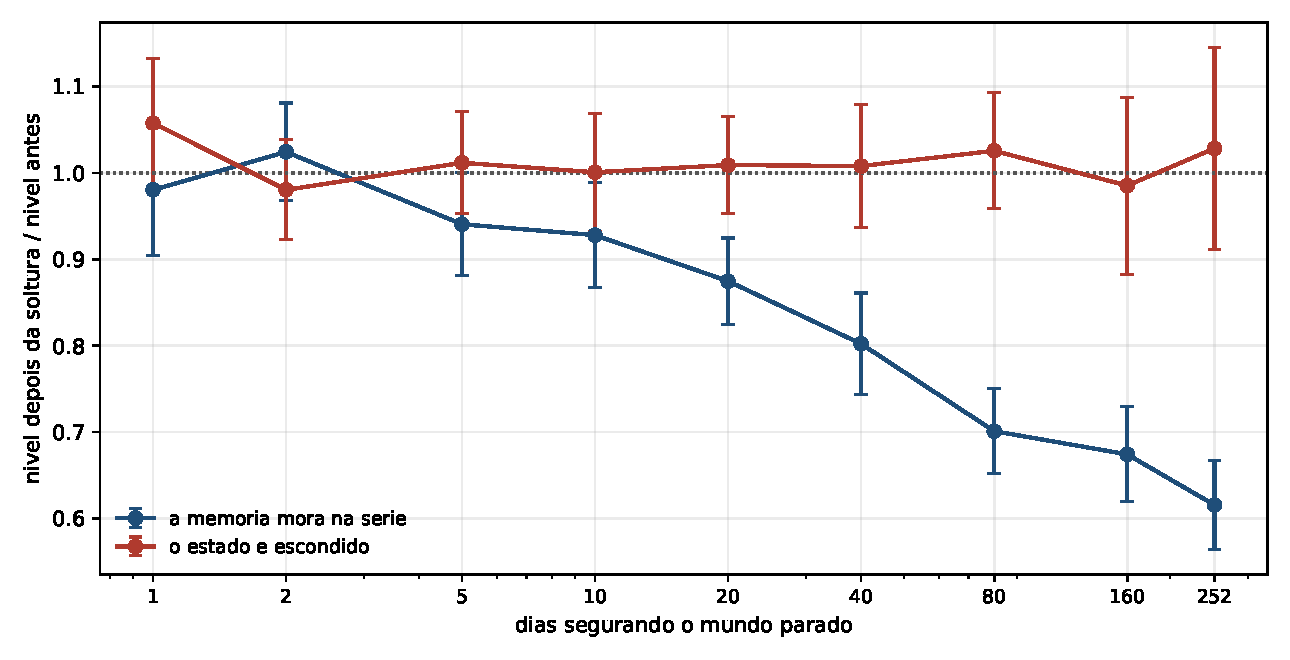
\includegraphics[width=\linewidth]{figuras/E10_desenho_da_intervencao_1.pdf}
  \caption{A resposta dos dois mundos contra o tempo de contenção, com as barras de dispersão
    desenhadas sobre \numDesenhoReplicatasPorCelula{} replicatas por ponto. A linha pontilhada é a
    resposta de um mundo que volta ao que era. O eixo horizontal é logarítmico, de modo que a
    distância entre as últimas marcas vale mais dias do que a figura sugere.}
  \label{fig:intervencao}
\end{figure}

\section{O preço de separar}

Com a resposta na mão, o preço sai de uma conta de duas linhas. Cada mundo carrega a sua dispersão
entre replicatas, e os dois intervalos de confiança precisam ficar separados: se a soma dos dois
raios tem de caber dentro da diferença que se quer ver, então
\[
n \;=\; \Big( \frac{z\, s}{d} \Big)^{2},
\]
onde $s$ é a soma dos dois desvios medidos, $z$ é o quantil da confiança declarada e $d$ é a
diferença que se insiste em ver. O preço em dias de experimento é $n$ vezes a duração de uma
replicata.

A conta tem uma exigência embutida que é fácil de esquecer: um desenho só vale onde a diferença
existe. Comprar replicatas para enxergar uma diferença que a contenção não produz é comprar um erro
de leitura, porque o experimento sairia dizendo que não há diferença, com toda a confiança do
mundo. Declarando \numDesenhoVinteCentesimosReplicatas{} replicatas para uma diferença de um quinto
do nível do mundo, o melhor desenho é a contenção de \numDesenhoVinteCentesimosContensao{} dias, ao
custo de \numDesenhoVinteCentesimosDias{} dias. Insistindo numa diferença maior, o desenho fica mais
barato: a contenção de \numDesenhoTrintaCentesimosContensao{} dias com
\numDesenhoTrintaCentesimosReplicatas{} replicatas custa \numDesenhoTrintaCentesimosDias{} dias.
Pedindo uma diferença de quinze centésimos do nível do mundo, o desenho mais barato encarece de
novo: contenção de \numDesenhoQuinzeCentesimosContensao{} dias,
\numDesenhoQuinzeCentesimosReplicatas{} replicatas e \numDesenhoQuinzeCentesimosDias{} dias de
experimento.

O melhor desenho de todos declara exatamente o que a contenção entrega, e é a linha de
\numDesenhoApertadoContensao{} dias da \cref{tab:resposta} que ganha: uma diferença de
\numDesenhoApertadoDiferenca{}, \numDesenhoApertadoReplicatas{} replicatas e
\numDesenhoApertadoDias{} dias de experimento. Segurar o mundo por um dia só custaria
\numDesenhoApertadoDiasCurta{} dias, e segurar por duzentos e cinquenta e dois custa
\numDesenhoCustoDuzentosECinquentaEDois{}. O ótimo é interior porque as duas pontas puxam para lados
opostos: contenção curta não produz diferença que valha a conta, contenção longa produz diferença
maior e ao mesmo tempo mais dispersão --- a soma dos dois desvios vai de \numDesenhoDesvioMenor{} a
\numDesenhoDesvioMaior{} ao longo da varredura ---, já que o estado escondido tem mais chance de
atravessar uma contenção longa e estragar a comparação entre replicatas.

\begin{figure}[htbp]
  \centering
  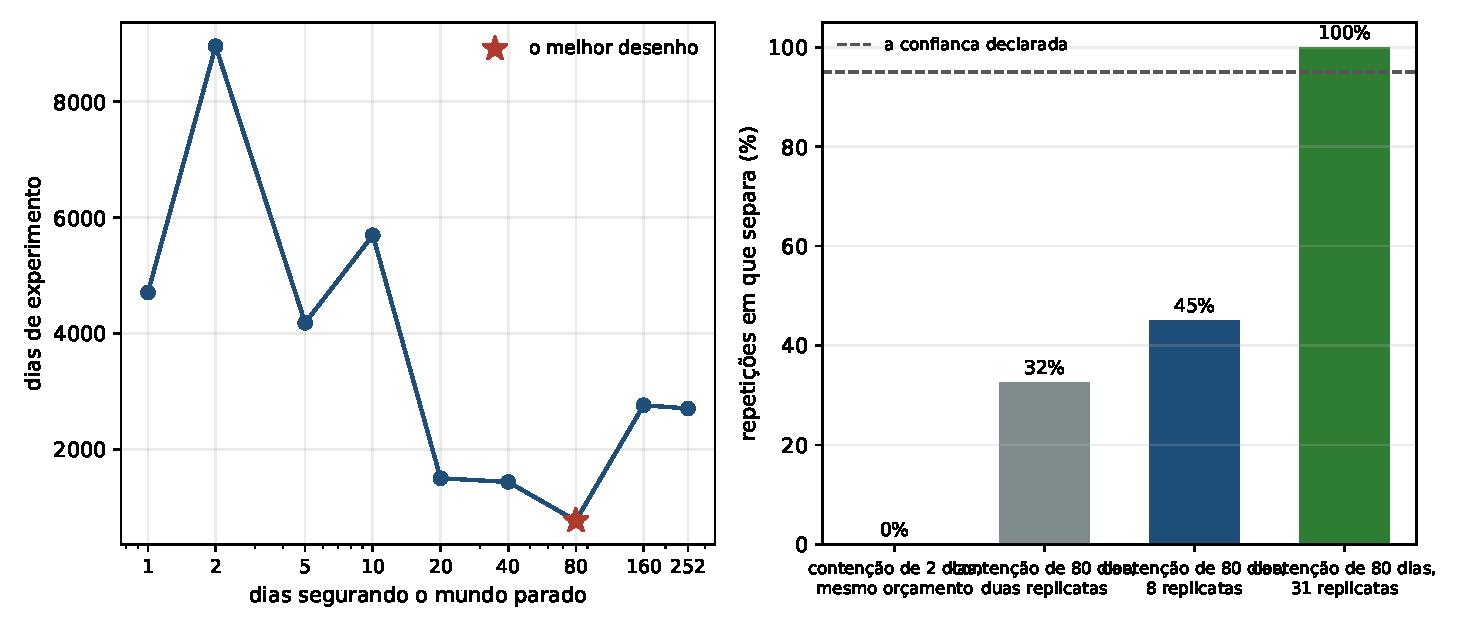
\includegraphics[width=\linewidth]{figuras/E10_desenho_da_intervencao_2.pdf}
  \caption{À esquerda, o preço do desenho que declara exatamente a diferença medida. À direita, a
    promessa do desenho verificada por repetição do experimento inteiro: a fração das repetições em
    que os dois intervalos de fato deixam de se cruzar.}
  \label{fig:preco_do_desenho}
\end{figure}

\section{A promessa do desenho, medida}

A conta acima promete \numDesenhoConfiancaPct\% de confiança, e essa promessa pode ser conferida:
basta repetir o experimento inteiro muitas vezes e contar em quantas delas os dois intervalos
deixam de se cruzar. Repetindo \numDesenhoMeta{} vezes, o desenho da conta separa em
\numDesenhoSeparaPlanejadaPct\% delas. A conta prometia \numDesenhoConfiancaPct\%.

O motivo da diferença está na resposta, e não na álgebra. A conta supõe que a média de um punhado
de replicatas se comporta como a média de muitos sorteios pequenos. A resposta do mundo de estado
escondido tem cauda gorda: às vezes um episódio agitado cobre a janela inteira do experimento, e
aquela replicata responde num nível que as outras não alcançam. Uma cauda dessas estraga a média
com poucas replicatas, e a conta não sabe disso.

O conserto é o que o próprio laboratório permite: dobrar e quadruplicar até a promessa se cumprir.
O dobro das replicatas separa em \numDesenhoSeparaDobroPct\%, e o quádruplo em
\numDesenhoSeparaQuadruploPct\%. O desenho que entrega a confiança declarada é o de
\numDesenhoEntregueReplicatas{} replicatas de \numDesenhoApertadoContensao{} dias, que separa em
\numDesenhoEntreguePct\% das repetições ao custo de \numDesenhoEntregueDias{} dias de experimento ---
perto de quatro vezes o preço da conta.

Fica a regra que este capítulo assina, e ela vale para qualquer desenho que venha depois:
\textbf{o preço de um desenho é medido, não calculado}. A conta diz onde procurar; a repetição diz
quanto custa.

\section{O mesmo orçamento no lugar errado}

Falta o controle que dá sentido ao número, e ele é o mesmo que fecha todos os capítulos deste
livro: gastar os mesmos dias na contenção errada. O desenho apertado custa
\numDesenhoApertadoDias{} dias; comprando com esse orçamento a contenção de dois dias, cabem
\numDesenhoMesmaContaReplicatas{} replicatas. Elas separam os dois mundos em
\numDesenhoSeparaCurtaPct\% das repetições do experimento inteiro.

O número faz sentido quando se olha a tabela: aos dois dias de contenção a diferença medida é
\numDesenhoDiferencaDois{}, de modo que nenhuma quantidade de replicatas compra o que a contenção
não produziu, e a única coisa que cresce com o orçamento é a certeza numa diferença que não existe.
O mesmo vale para o experimento do início do capítulo, o de segurar muito tempo e olhar duas vezes.

\section{O que fica}

Fica a segunda resposta da travessia. A intervenção separa as duas explicações que a observação
empatou, e o preço está medido: milhares de dias de experimento, distribuídos em replicatas de
contenção e espera. Fica com ela a forma da conta, que vai servir a qualquer travessia seguinte ---
declarar a diferença que se quer ver, medir a dispersão, comprar replicatas até a promessa se
cumprir, e conferir a promessa por repetição, porque a cauda gorda mente para a álgebra.

Fica também o limite, e ele é duro. Uma intervenção dessas existe para um sistema que se pode
segurar: uma rede, uma máquina, uma planta, um serviço. Para um índice de mercado ela não existe, e
o que o dado não tem não se compra com confiança. A travessia decide entre explicações onde há uma
alavanca, e onde não há, o empate permanece.

O fracasso seguinte está no próprio preço. Os dias de experimento gastos segurando o mundo são dias
em que o sistema fica parado, e um sistema parado é um sistema que não está aprendendo nada de novo
--- nem sobre o mundo, nem sobre o próprio modelo. Se o orçamento é um só, proteger e aprender
disputam a mesma moeda, e nada do que foi construído até aqui disse quem paga a conta.
